\includepdf[pages=-]{"Tareas/Hoja 3/Hoja 3"}
\begin{enumerate}[label=\color{red}\textbf{\arabic*)}, leftmargin=*]
	\item \lb{Un experimento aleatorio puede terner cuatro resultados diferentes $\Omega=\{a,b,c,d\}$. Estudiar si las siguientes asignaciones de probabilidad pueden ser correctas:}
	
	\begin{center}
		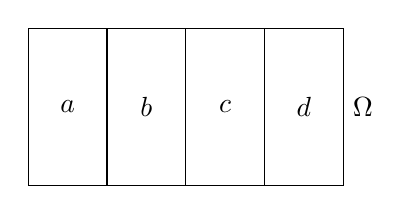
\begin{tikzpicture}
			\foreach \x in {0,...,3}{
			\draw (\x,0) rectangle ({\x+1},2);
			}
			
			\node at (0.5,1) {$a$};
			\node at (1.5,1) {$b$};
			\node at (2.5,1) {$c$};
			\node at (3.5,1) {$d$};
			\node[right] at (4, 1) {$\Omega$};
		\end{tikzpicture}
	\end{center}
	\begin{enumerate}[label=\color{red}\alph*)]
		\item \db{$P(a)=0.1,P(b)=0.3,P(c)=0.4$ y $P(d)=0.2$}
		
		Es correcto porque suma 1.
		\item \db{$P(a)=\dfrac{1}{5},P(b)=\dfrac{1}{5},P(c)=\dfrac{1}{5}$ y $P(d)=\dfrac{1}{4}$}
		
		No suma 1 $\longrightarrow$ No es correcto
		
		\item \db{$P(a)=0.6,P(b)=-0.2,P(c)=0.4$ y $P(d)=1.2$}
		
		$P(b)$ tiene valor negativo $\longrightarrow$ No es correcto
		
		\item \db{$P(a)=\dfrac{1}{5},P(b)=\dfrac{1}{4},P(c)=\dfrac{1}{3}$ y $P(d)=\dfrac{1}{6}$}
		
		No suma 1 $\longrightarrow$ No es correcto
	\end{enumerate}
	\item \lb{Si $A,B,C$ y $D$ son cuatro sucesos mutuamente excluyentes de un espacio de probabilidad $(\Omega,\mathcal{S},P)$, estudiar si las siguientes asignaciones pueden ser correctas:}
	
	\begin{figure}[!ht]
		\centering
		\resizebox{0.3\textwidth}{!}{%
			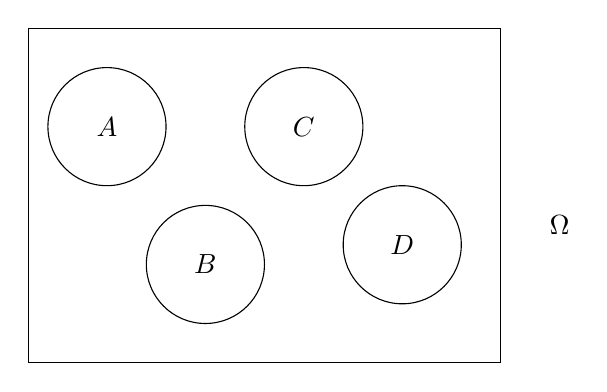
\begin{tikzpicture}
				\draw  (1.5,13.5) circle (0.75cm) node {$A$} ;
				\draw  (2.75,11.75) circle (0.75cm) node {$B$} ;
				\draw  (4,13.5) circle (0.75cm) node {$C$} ;
				\draw  (5.25,12) circle (0.75cm) node {$D$} ;
				\draw  (0.5,14.75) rectangle (6.5,10.5);
				\node  at (7.25,12.25) {$\Omega$};
			\end{tikzpicture}
		}%
	\end{figure}
	
	Debe cumplirse $P(i)\ge0\;\forall i=A,B,C,D$ y $P(A)+P(B)+P(C)+P(D)\le1$
	\begin{enumerate}[label=\color{red}\alph*)]
		\item \db{$P(A)=0.1,P(B)=0.3,P(C)=0.4$ y $P(D)=0.2$}
		
		Si es correcta
		\item \db{$P(A)=\frac{1}{5},P(B)=\frac{1}{5},P(C)=\frac{1}{5}$ y $P(D)=\frac{1}{4}$}
		
		$\sum_{i=A,\dots,D}p(i)=\dfrac{1}{5}+\dfrac{1}{5}+\dfrac{1}{5}+\dfrac{1}{4}=\dfrac{17}{20}<1$. Si es correcta
		\item \db{$P(A)=0.6,P(B)=-0.2,P(C)=0.4$ y $P(D)=1.2$}
        
        No es correcta porque $P(B)=-0.2<0$
		\item \db{$P(A)=\frac{1}{5},P(B)=\frac{1}{4},P(C)=\frac{1}{3}$ y $P(D)=\frac{1}{2}$}
        
        $\sum_{i=A,\dots,D}p(i)=\dfrac{1}{5}+\dfrac{1}{4}+\dfrac{1}{3}+\dfrac{1}{2}=\dfrac{77}{60}>1\longrightarrow$ No es correcta (pero sí en el apartado \lb{(e)} sí lo es.)
        \item \db{Responder a las cuatro cuestiones anteriores suponiendo que los sucesos $A$, $B, C$ y $D$ no son mutuamente excluyentes.}
	\end{enumerate}
    \item \lb{Poner un ejemplo de un espacio de probabilidad donde $\mathcal{S}\neq\wp(\Omega)$}
    
    $\mathrm{Exp}=$"Lanzar un dado".$\Omega=\{1,2,3,4,5,6\}$\\
    $A=$"Obtener número par"\\
    $\mathcal{S}=\{\omega,\varnothing,A,A^c\}$ es una $\sigma$-álgebra.\\
    $\mathcal{S}\subseteq P(\Omega)$
    \item \lb{Construir el conjunto de sucesos $S$ de un espacio de probabilidad sabiendo que $A,B\in S$. Calcular $P(A)$ y $P(B)$ sabiendo que $P(A\cup B)=\dfrac{3}{5},P(A\cap B)=\dfrac{1}{5}$ y $P(A-B)=\dfrac{1}{5}$.}
    
    $A,B\in\mathcal{S}$\\
    $\mathcal{S}=\{\Omega,\varnothing,A,B,A^c,B^c,A\cup B,A\cap B,A^c\cap B^c,A^c\cup B^c,A\cap B^c,B\cap A^c,A\cup B^c,B\cup A^c,A\triangle B,(A\triangle B)^c\}$\\
    $P(A\cup B)=\dfrac{3}{5},P(A\cap B)=\dfrac{1}{5},P(A-B)=\dfrac{1}{5}$ ¿$P(A)$ y $P(B)$?
    \begin{itemize}[label=$-$]
    \item $\lbb{P(A\cup B)}{\frac{3}{5}}=P(A)+P(B)-\lbb{P(A\cap B)}{\frac{1}{5}}\longrightarrow P(B)=\frac{2}{5}$
    \item $\lbb{P(A-B)}{\frac{1}{5}}=P(A)-\lbb{P(A\cap B)}{\frac{1}{5}}\longrightarrow P(A)=\frac{2}{5}$
    
    	\begin{tikzpicture}
    		\draw[fill=lightblue, opacity=0.5] (0,0) circle (1.5cm) ;
    		\draw[fill=red, opacity=0.5] (2,0) circle (1.5cm) ;
    		\draw (0,0) circle (1.5) node[above] {$A$};
    		\draw (2,0) circle (1.5) node[above] {$B$};
            \node at (4,0) {$\Omega$};
    	\end{tikzpicture}
    \end{itemize}
    \item \lb{Sean $P(A),P(B),P(A\cap B)$ las probabilidades de los sucesos $A,B,A\cap B$, respectivamente. Determinar en función de ellas:}
    \begin{enumerate}[label=\color{red}\alph*)]
    	\item $\db{P(A\cap\overline{B})}$
        
        $P(A\cap \overline{B})=P(A-B)=P(A)-P(A\cap B)$
        \item $\db{P(\overline{A}\cap B)}$
        
        $P(\overline{A}\cap B)=P(B-A)=P(B)-P(A\cap B)$
    \end{enumerate}
    \item \lb{Se lanzan dos monedas al azar.}
    \begin{enumerate}[label=\color{red}\alph*)]
    	\item \db{Calcula la probabilidad de que ambas monedas muestren cara después del lanzamiento.}
        
        Experimento aleatorio: "Observar el resultado de lanzar 2 monedas".\\
        $C_i=$"Ha salido cara en la moneda $i$", $i=1,2$
        $+_i=$"Ha salido cruz en la moneda $i$", $i=1,2$\\
        $\Omega=\left\{\{C_1,C_2\},\{C_1,+_2\},\{+_1,C_2\},\{+_1,+_2\}\right\}\longrightarrow$\begin{minipage}[l]{4cm}
        Espacio muestral finito con 4 elementos (4 sucesos elementales equiprobables).
        \end{minipage}\\
                $P(C_1,C_2)=\dfrac{1}{4}$
        \item \db{Calcular la probabilidad de obtener al menos una cara.}
        $P(\Omega-\{x_1,x_2\})=P\overline{(+_1,+_2)}=1-P(+_1,+_2)=1-\dfrac{1}{4}=\dfrac{3}{4}$
    \end{enumerate}
    \lb{Nota: En todos los problemas en que se manejan bolas, urnas, dados, monedas, etc. estos objetos son distintos mientras no se diga lo contrario.}
    \item \lb{De una baraja francesa (52 cartas) se sacan al azar tres cartas. Se pide:}
    \begin{enumerate}[label=\color{red}\alph*)]
    	\item \db{La probabilidad de que en las tres cartas extraídas al azar haya exactamente un as.}
        
        Experimento aleatorio: "Observar el resultado al extraer 3 cartas de la baraja"\\
        $\Omega=\left\{\{3_T,2_E,1_P\},\{1_E,1_T,!_p\},\dots\right\}\longrightarrow$\begin{minipage}[l]{6cm}
        Espacio muestra finito. Todas las sucesiones son equiprobables.
        \end{minipage}
        
       ¿Cuántas hay? $|\Omega|=$ casos posibles\qquad\lb{(aplico definición de Laplace)}\\
        $|\Omega|=\dbinom{52}{3}=\dfrac{52!}{3!(52-3)!}=22100$ n\textdegree de casos posibles\\
        P("Exactamente un as")$=\dfrac{\text{n\textdegree de casos favorables}}{n\textdegree casos posibles}=\dfrac{4512}{22100}\simeq0.2$\\
        n\textdegree casos posibles$=\dbinom{4}{1}\cdot\dbinom{48}{2}=4512$
        \item \db{La probabilidad de que en las tres cartas extraídas haya al menos un as.}
        
        P("Haya al menos 1 as")=1-P("No haya ningún as")=$1-0.78=0.22$\\
        P("No haya ningún as")$=\dfrac{\binom{48}{3}}{\binom{52}{3}}\simeq0.78$
    \end{enumerate}
    \item \lb{Se toman al azar 4 cartas de una baraja española (que se compone de 40 cartas distribuidas en 4 palos: oros, copas, bastos y espadas). Se pide la probabilidad de que:}
    \begin{enumerate}[label=\color{red}\alph*)]
    	\item \db{Ninguna de las 4 cartas sean de oros.}
        
        Exp. aleatorio="Obtener el resultado de extraer 4 cartas de la baraja"\\
        $\Omega=\left\{\{3_C,1_O,2_E,4_B\},\dots\right\}\longrightarrow$Espacio finito. Todas las sucesiones son equiprobables. \lb{(aplico definición de Laplace)}\\
        $\Omega=\binom{40}{4}$ nº de casos posibles\\
        P("Ninguna sea Oros")$=\dfrac{\text{nº de casos favorables}}{nº casos posibles}=\dfrac{\binom{30}{4}}{\binom{40}{4}}\simeq1.24$
        \item \db{Exactamente una de las cartas sea de oros.}
        
        P("Exactamente un oro")$=\dfrac{\binom{10}{1}\cdot\binom{30}{3}}{\binom{40}{4}}\simeq0.44$
        \item \db{Sean las 4 de oros.}
        
        P("Sean las 4 oros")$=\dfrac{\binom{10}{4}}{\binom{40}{4}}\simeq0.0023$
        \item \db{Sean las 4 de palos distintos.}
        
        P("Sean 4 palos distintos")$=\dfrac{\binom{10}{1}\cdot\binom{10}{1}\cdot\binom{10}{1}\cdot\binom{10}{1}}{\binom{40}{4}}\simeq0.11$
    \end{enumerate}
    \item \lb{Una baraja francesa tiene 52 cartas, 26 rojas (los corazones y los diamantes) y 26 negras (picas y tréboles). Se divide la baraja (al azar) en dos partes iguales (26 cartas en cada parte). Calcular la probabilidad de que en cada parte haya igual número de cartas negras que de rojas.}
    
    Exp. aleatorio = ("Observar el resultado de separar 2 montones de 26 cartas").
    
    $\Omega=\left\{\{\text{Roja}\oplus\text{Negras}\},\{\text{DiaTreb}\oplus\text{PieCora},\dots\}\right\}\longrightarrow$ Espacio muestral finito. Todas las sucesiones son equiprobables. \lb{(Laplace)}
    
    ¿Cuántas hay? $|\Omega|=$ casos posibles\\
    $|\Omega|=\binom{52}{26}$ nº casos posibles.\\
    P("Haya el mismo nº de cartas negras y rojas en cada montón")$=\dfrac{\text{nº de casos favorables}}{\text{nº de casos posibles}}=\dfrac{\binom{26}{13}\cdot\binom{26}{13}}{\binom{52}{26}}\sim0.212\equiv$P("13 rojas y 13 negras en cada una de las partes")
    \item \lb{En un sobre hay veinte papeletas, ochos llevan dibujando un coche y el resto están en blanco. Hallar la probabilidad de extraer al menos una papeleta con el dibujo de un coche si:}
    
    20 papeletas$\left\langle\begin{tabular}{l}
    8 coches\\
    12 blancos
    \end{tabular}\right.$
    \begin{enumerate}[label=\color{red}\alph*)]
    	\item \db{Se saca sólo una papeleta.}
        
        P("No coche")$=\dfrac{\text{nº de casos favorables}}{\text{nº de casos posibles}}=\dfrac{12}{20}=\dfrac{3}{5}$\\
        P("Al menos un coche")=1-P("No salga ningún coche")=$1-\dfrac{3}{5}=\dfrac{2}{5}=0.4$
        \item \db{Se extraen dos papeletas.}
        
        P("No coche")=$\dfrac{\binom{12}{2}}{\binom{20}{2}}\simeq0.35$\\
        P("Al menos un coche")=$1-0.35=0.65$
        \item \db{Se extraen tres papeletas.}
        
        P("No coche")=$\dfrac{\binom{12}{3}}{\binom{20}{3}}\simeq0.19$\\
        P("Al menos un coche")=$1-0.19=0.81$
    \end{enumerate}
    \item \lb{Cuatro matrimonios se reúnen a comer y se sientan al azar en las 8 sillas que hay alrededor de una mesa redonda sin que queden huevos entre dos sillas.}
    \begin{enumerate}[label=\color{red}\alph*)]
    	\item \db{Calcular la probabilidad de que cada caballero quede junto a su esposa.}
        
        \begin{wrapfigure}{l}{0.3\textwidth}
        \begin{tikzpicture}
        \draw (0,0) circle (2);
        \node[above] at (90:2) {1};
        \node[above right] at (45:2) {2};
        \node[right] at (0:2) {3};
        \node[below right] at (315:2) {4};
        \node[below] at (270:2) {5};
        \node[below left] at (225:2) {6};
        \node[left] at (180:2) {7};
        \node[above left] at (135:2) {8};
        \end{tikzpicture}
        \end{wrapfigure}
        
        Experimento aleatorio="Observar en qué silla se situan los 4 caballero y sus esposas al disponerlos aleatoriamente".
        
        4 caballeros y 4 esposas$\left\langle\begin{array}{l}
        c_1,c_2,c_3,c_4\\
        e_1,e_2,e_3,e_4
        \end{array}\right.$
        
        $\Omega=\left\{(c_1,c_2,c_3,c_4,e_1,e_2,e_3,e_4),\dots,(e_1,e_2,e_3,e_4,c_1,c_2,c_3,c_4)\right\}\longrightarrow$ Aplico Laplace\\
        P("Cada caballero con su esposa")=$\dfrac{\text{Casos favorables}}{\text{Casos posibles}}=\dfrac{2\cdot4!\cdot2^4}{8!}=\dfrac{2}{105}$\\
        \begin{itemize}[label=\color{lightblue}$-$, leftmargin=*]
        	\item \underline{Casos favorables:} Los matrimonios (4) podrán sentarse juntos en las sillas $\{1,2\},\{3,4\},\{5,6\},\{7,8\}$ de $4!$ formas y además hay 2 opciones de sentar a cada matrimonio en un par de sillas.
            \item Observarr que tenemos el mismo escenario para los pares de sillas $\{8,1\},\{2,3\},\{4,5\},\{6,7\}$.
        \end{itemize}
        \item \db{Calcular la probabilidad de que queden alternados las señoras y los caballeros, o sea, cada señora quede entre dos caballeros.}
        
        P("Cada señora entre 2 caballeros")=$\dfrac{2\cdot4!\cdot4!}{8!}=\dfrac{1}{35}$\\
        \underline{Casos favorables:} Tenemos las siguientes opciones:
        \begin{enumerate}[label=\color{lightblue}\arabic*)]
        	\item Todas las señoras a las sillas impares y los caballeros en las pares $\underbrace{\{1,3,5,7\}}_{\text{Señoras}},\underbrace{\{2,4,6,8\}}_{\text{Caballeros}}$
            
            \lb{Ambos se pueden colocar de $4!$ formas distintas}
            \item Análogo, pero sillas impares para caballeros.
        \end{enumerate}
    \end{enumerate}
    \item \begin{enumerate}[label=\color{red}\alph*)]
    	\item \lb{¿Cuál es la probabilidad de que en un aula con 25 alumnos nunca coincidan sus cumpleaños?}
        \item \lb{¿Cuál es la probabilidad de que en un aula con 25 alumnos, al menos coincidan dos cumpleaños?}
    \end{enumerate}
    \item \lb{Supongamos que lanzamos un dado dos veces:}
    \begin{enumerate}[label=\color{red}\alph*)]
    	\item \db{¿Cuál es la probabilidad de que la suma de los puntos obtenidos sea igual a 8?}
        \item \db{¿Cuál es la probabilidad de que la suma de los puntos obtenidos sea igual a 9?}
    \end{enumerate}
\end{enumerate}
